\documentclass[]{article}
\usepackage{amsmath}
\usepackage{authblk}
\usepackage{caption}
\usepackage{graphicx}
\usepackage{longtable}

\graphicspath{ {/home/daniel/Code/puc/} }
\usepackage{multicol}

\usepackage[a4paper, total={6in, 8in}]{geometry}

%opening
\title{Relatório 2 - Medida de similaridade para dados categórios ordinais sem matching}
\author[1]{Daniel Schlickmann Bastos}
\date{09/03/2021}

\begin{document}
	\maketitle
	
	\section{Introdução}
	
	Dado as duas medidas exploradas anteriormente (1 e 2, brevemente explicadas abaixo), a primeira sendo em relação à valorizaçã0 dos atributos pela empresa e a segunda, o mérito de cada candidado dado o seu nível de conhecimento nos atributos, uma terceira medida incorporando as duas está sendo proposta nesse relatório.
	
	Recapitulando, a primeira medida
	
	\begin{center}
		\begin{equation}
			S_j = \dfrac{\sum_{k = 0}^N \frac{r_{jk}}{|L| - 1}}{N}
		\end{equation}	
	\end{center}
	
	apresenta uma forma de medir o nível de valorização de cada atributo de empresas por meio de média simples dos valores numéricos correpondentes à cada atributo.
	
	Nela, $L$ representa o conjunto de níveis de conhecimento ($\{$ nada, básico, intermediário, avançado $\}$) e $r_{jk}$, o nível de valorização ordinal pela empresa $j$ do atributo $k$ $(0, 1, 2, 3)$ para cada item, respectivamente, em $L$.
	
	Já a segunda medida, apresentada no relatório anterior, diz o mérito de cada candidato dado o seu nível de conhecimento em cada atributo, porém, tomando como verdade que todos os atributos têm a mesma relevância para a empresa. 
	
	\begin{center}
		\begin{equation}
			S_i = \dfrac{\sum_{k = 0}^N \dfrac{r_{ik}}{|L| - 1} * C^{r_{ik} - (|L| - 1)}}{\sum_{k = 0}^N C^{r_{ik} - (|L| - 1)}}
		\end{equation}		
	\end{center}
	
	onde $r_{jk}$ é o nível de conhecimento ordinal do candidato $i$ do atributo $k$, $(0, 1, 2, 3)$ para cada item, respectivamente, em $L$. $ C $ é um valor que determina quanto mérito cada nível de conhecimento terá, e fica a cargo do usuário a determinar seu valor numérico a partir de seu contexto.
	
	\section{Proposta}
	
	\begin{center}
		\begin{equation}
			S_{ij} = \dfrac{\sum_{k = 0}^N \dfrac{r_{ik}*(r_{jk} + 1)}{|L|^2 - |L|} * C^{r_{ik} - (|L| - 1)}}{\sum_{k = 0}^N C^{r_{ik} - (|L| - 1)}}
		\end{equation}	
	\end{center}
	
	Para compreendê-la melhor, o seu processo de derivação será explicado.
	
	Partimos da ideia que a valorização do conhecimento é linear, portanto, tanto a valorização da empresa quanto o conhecimento do candidato nos respectivos atributos terão um comportamento linear. A operação matemática que combina as duas medidas da melhor forma é a multiplicação, e na fórmula é representada por $ r_{ik}*(r_{jk} + 1)/ (|L|^2 - |L|) $. 
	
	Ao invés de ser $ (r_{ik}*r_{jk})/((|L| - 1)*(|L| - 1)) $, o valor da valorização da empresa é modificado para que no numerador e denominador haja uma adição de $1$. Isso foi feito para contornar a situação de uma valorização nula pela empresa $r_{jk} = 0$, onde sem a adição, qualquer nível de conhecimento do candidato seria desvalorizado totalmente e casos como um conhecimento "avançado" ter uma valorização igual, mesmo que nula, à "básico" surgiria, o que não é correto, pois é necessário distinguir conhecimentos maiores de menores. Portanto, ao realizar a adição, tem-se
	
	\begin{center}
		\begin{equation}
			\dfrac{r_{ik}*(r_{jk} + 1)}{(|L| - 1)*(|L| - 1 + 1)} = \dfrac{r_{ik}*(r_{jk} + 1)}{|L|^2 - |L|}
		\end{equation}	
	\end{center}
	
	Desta maneira, resta integrar uma medida de mérito. Ao incorporar o valor de mérito de certo conhecimento com o valor de valorização e conhecimento de um atributo (equação 3), é formada a medida
	
	
	\begin{center}
		\begin{equation}
			\dfrac{r_{ik}*(r_{jk} + 1)}{|L|^2 - |L|} * C^{r_{ik} - (|L| - 1)}
		\end{equation}
	\end{center}
	
	
	porém, como é nessário manter os valores entre $0$ e $1$, a média ponderada é tirada. O valor do mérito corresponderá ao peso de cada valor de valorização e conhecimento. Por fim, chega-se na medida sendo proposta:
	
	\begin{center}
		\begin{equation}
			S_{}ij = \dfrac{\sum_{k = 0}^N \dfrac{r_{ik}*(r_{jk} + 1)}{|L|^2 - |L|} * C^{r_{ik} - (|L| - 1)}}{\sum_{k = 0}^N C^{r_{ik} - (|L| - 1)}}
		\end{equation}	
	\end{center}
	
	\subsection{Interpretação e Visualização}
	
	Para compreender melhor a relação entre a valorização e conhecimento, e mérito de um atributo, o gráfico abaixo é utilizado. O eixo x é o nível de conhecimento ($r_{ik}$) variando de $0$ à $3$, e o $y$, o conhecimento incorporado com o mérito (equação 5). Nele, $C$ está igual à $2$.
	
	Cada curva representa o comportamento de cada nível de valorização, a mais baixa, $f_{r_{jk} = 0}$, ou $f_0$, apresenta o comportamento de uma valorização nula ($0$) de um atributo, já a de cima, $f_1$, apresenta o comportamento de uma valorização básico ($1$), $f_2$, a de uma valorização intermediária ($2$), e a $f_3$, uma valorização avançada ($3$).
	
	As equações de cada curva são as seguintes para o cenário de 4 níveis de conhecimento e valorização (nada - 0, básico - 1, intermediário - 2 e avançado - 3)
	
	\begin{center}
		$ f_{r_{jk} = 3}(x) = \dfrac{x*(3 + 1)}{4^2 - 4} * 2^{x - 3} $
		
		$ f_{r_{jk} = 2}(x) = \dfrac{x*(2 + 1)}{4^2 - 4} * 2^{x - 3} $
		
		$ f_{r_{jk} = 1}(x) = \dfrac{x*(1 + 1)}{4^2 - 4} * 2^{x - 3} $
		
		$ f_{r_{jk} = 0}(x) = \dfrac{x*(0 + 1)}{4^2 - 4} * 2^{x - 3} $
	\end{center}
	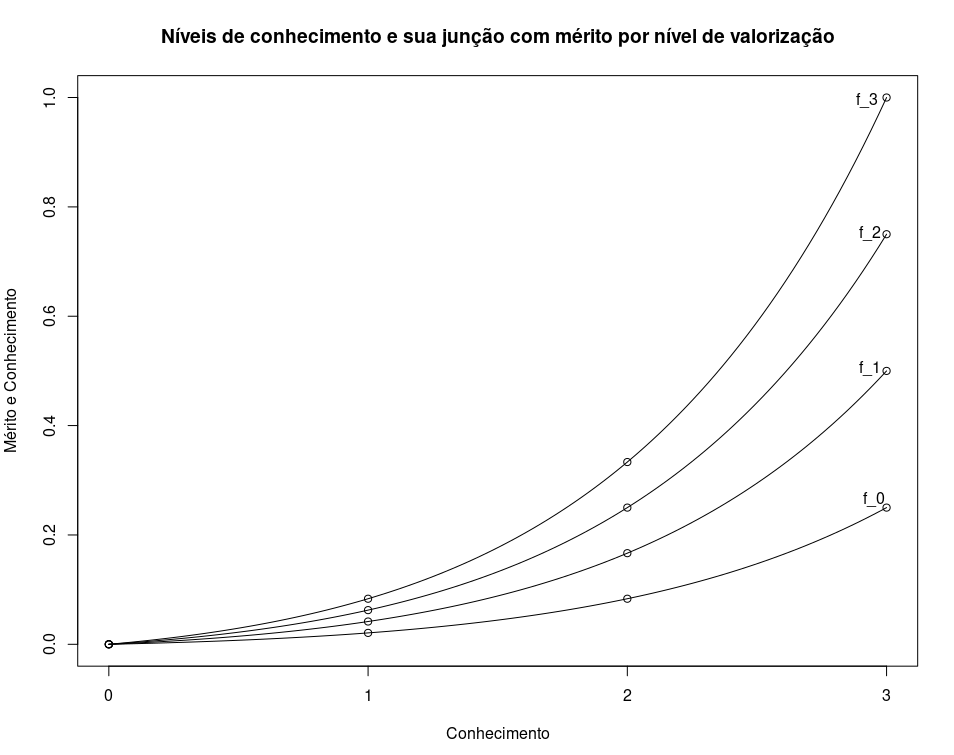
\includegraphics[width=13.2cm, height=8cm]{plot}
	
	Intepretando um caso nesse gráfico: dado um certo atributo, PPT, por exemplo, onde a valorização é de um nível nulo (função $f_0$) pela empresa e um candidado com nível de conhecimento avançado ($x = 3$), a junção do mérito e conhecimento dado essa valorização é aproximadamente $0.2$. Já um outro caso onde um atributo Excel, por exemplo, tem um nível de valorização avançado pelo empresa ($f_3$) e um candidato com nível de conhecimento intermediário ($x = 2$), a junção do mérito e conhecimento é aproximadamente $0.3$
	
	Caso a quantidade de mérito por nível queira ser aumentada, o valor de $C$ é o que tem que ser diminuído. Alterando-o agora para 1.2, temos o seguinte gráfico:
	
	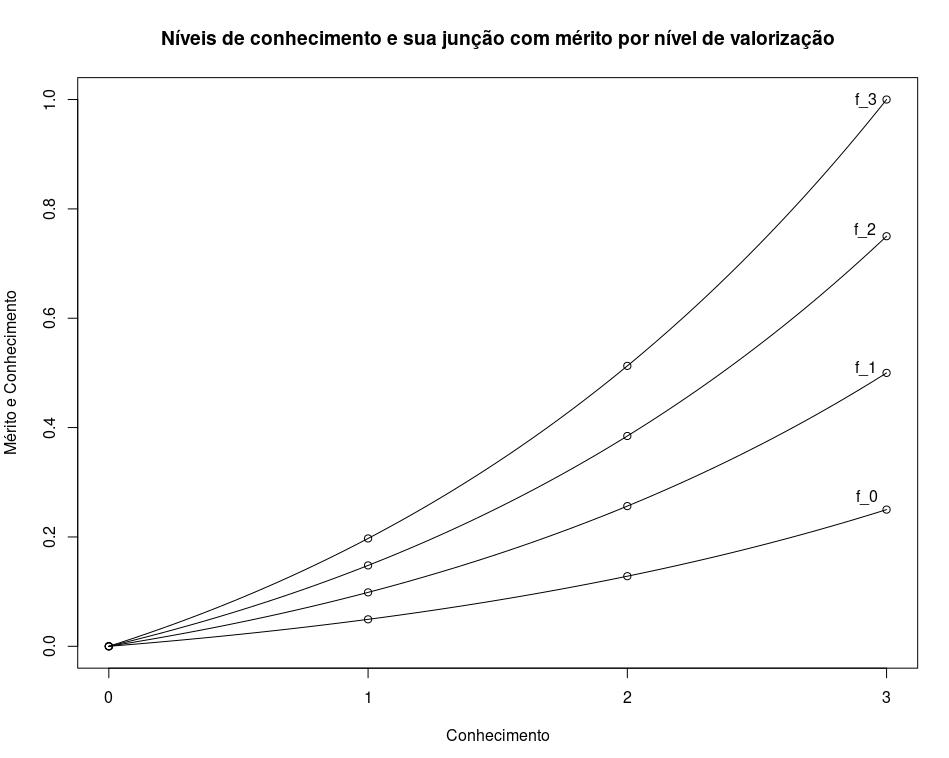
\includegraphics[width=13.2cm, height=8cm]{plot-2}
	
	Desse modo, o mesmo cenário anterior resultará no mesmo valor para o primeiro caso ($y \approx 0.2$), porém para o segundo ($y \approx 0.3$), o valor de $y$ aumenta para aproximadamente $0.5$, ou seja, o mérito dos conhecimentos intermediários aumentaram -- os dos básicos também.
	
	\section{Experimento}
	
	Para as 64 combinações de níveis de conhecimento de 3 atributos (Word, PPT e Excel) com níveis de valorização, foi calculado o valor de similaridade ($S_{ij}$) utilizando a equação 3.
	
	Para somente as seguintes combinações de níveis de valorização de cada atributo foram calculados os resultados.
	
	\begin{itemize}
		\item Excel = Avançado, PPT = Avançado, Word = Avançado
		\item Excel = Nada, PPT = Intermediário, Word = Avançado
		\item Excel = Nada, PPT = Nada, Word = Avançado
		\item Excel = Nada, PPT = Nada, Word = Nada
	\end{itemize}
	
	\section{Resultados}
	
	
	\begin{longtable}{|llll|r|} 
		\caption{Excel = Avançado, PPT = Avançado, Word = Avançado}
		\label{variability_impl_mech}
		\endfirsthead
		\endhead
		
		\hline
		{} & Excel     & PPT       & Word      & Similaridade \\
		\hline
		0  & nada      & nada      & nada      & 0.000000     \\
		1  & nada      & nada      & básico   & 0.142857     \\
		2  & nada      & básico   & nada      & 0.142857     \\
		3  & básico   & nada      & nada      & 0.142857     \\
		4  & nada      & básico   & básico   & 0.250000     \\
		5  & básico   & nada      & básico   & 0.250000     \\
		6  & básico   & básico   & nada      & 0.250000     \\
		7  & básico   & básico   & básico   & 0.333333     \\
		8  & nada      & nada      & médio    & 0.352941     \\
		9  & nada      & médio    & nada      & 0.352941     \\
		10 & médio    & nada      & nada      & 0.352941     \\
		11 & nada      & básico   & médio    & 0.421053     \\
		12 & nada      & médio    & básico   & 0.421053     \\
		13 & básico   & nada      & médio    & 0.421053     \\
		14 & básico   & médio    & nada      & 0.421053     \\
		15 & médio    & nada      & básico   & 0.421053     \\
		16 & médio    & básico   & nada      & 0.421053     \\
		17 & básico   & médio    & básico   & 0.476190     \\
		18 & médio    & básico   & básico   & 0.476190     \\
		19 & básico   & básico   & médio    & 0.476190     \\
		20 & nada      & médio    & médio    & 0.545455     \\
		21 & médio    & nada      & médio    & 0.545455     \\
		22 & médio    & médio    & nada      & 0.545455     \\
		23 & básico   & médio    & médio    & 0.583333     \\
		24 & médio    & básico   & médio    & 0.583333     \\
		25 & médio    & médio    & básico   & 0.583333     \\
		26 & nada      & nada      & avançado & 0.627907     \\
		27 & nada      & avançado & nada      & 0.627907     \\
		28 & avançado & nada      & nada      & 0.627907     \\
		29 & nada      & básico   & avançado & 0.659574     \\
		30 & nada      & avançado & básico   & 0.659574     \\
		31 & básico   & nada      & avançado & 0.659574     \\
		32 & básico   & avançado & nada      & 0.659574     \\
		33 & avançado & nada      & básico   & 0.659574     \\
		34 & avançado & básico   & nada      & 0.659574     \\
		35 & médio    & médio    & médio    & 0.666667     \\
		36 & básico   & básico   & avançado & 0.686275     \\
		37 & básico   & avançado & básico   & 0.686275     \\
		38 & avançado & básico   & básico   & 0.686275     \\
		39 & nada      & médio    & avançado & 0.735849     \\
		40 & nada      & avançado & médio    & 0.735849     \\
		41 & médio    & nada      & avançado & 0.735849     \\
		42 & médio    & avançado & nada      & 0.735849     \\
		43 & avançado & nada      & médio    & 0.735849     \\
		44 & avançado & médio    & nada      & 0.735849     \\
		45 & básico   & médio    & avançado & 0.754386     \\
		46 & básico   & avançado & médio    & 0.754386     \\
		47 & médio    & básico   & avançado & 0.754386     \\
		48 & avançado & básico   & médio    & 0.754386     \\
		49 & médio    & avançado & básico   & 0.754386     \\
		50 & avançado & médio    & básico   & 0.754386     \\
		51 & médio    & médio    & avançado & 0.809524     \\
		52 & médio    & avançado & médio    & 0.809524     \\
		53 & avançado & médio    & médio    & 0.809524     \\
		54 & nada      & avançado & avançado & 0.870968     \\
		55 & avançado & nada      & avançado & 0.870968     \\
		56 & avançado & avançado & nada      & 0.870968     \\
		57 & básico   & avançado & avançado & 0.878788     \\
		58 & avançado & básico   & avançado & 0.878788     \\
		59 & avançado & avançado & básico   & 0.878788     \\
		60 & médio    & avançado & avançado & 0.916667     \\
		61 & avançado & médio    & avançado & 0.916667     \\
		62 & avançado & avançado & médio    & 0.916667     \\
		63 & avançado & avançado & avançado & 1.000000     \\
		\hline
	\end{longtable}
	
	
	
	\begin{longtable}{|llll|r|}
		\caption{Excel = Nada, PPT = Intermediário, Word = Avançado}
		\label{variability_impl_mech}
		\endfirsthead
		\endhead
		
		\hline
		{} & Excel     & PPT       & Word      & Similaridade \\
		\hline
		0  & nada      & nada      & nada      & 0.000000     \\
		1  & básico   & nada      & nada      & 0.029570     \\
		2  & médio    & nada      & nada      & 0.062825     \\
		3  & nada      & básico   & nada      & 0.088710     \\
		4  & avançado & nada      & nada      & 0.099895     \\
		5  & básico   & básico   & nada      & 0.114583     \\
		6  & nada      & nada      & básico   & 0.118280     \\
		7  & básico   & nada      & básico   & 0.143229     \\
		8  & médio    & básico   & nada      & 0.144008     \\
		9  & médio    & nada      & básico   & 0.171702     \\
		10 & avançado & básico   & nada      & 0.177135     \\
		11 & nada      & médio    & nada      & 0.188474     \\
		12 & nada      & básico   & básico   & 0.200521     \\
		13 & avançado & nada      & básico   & 0.203852     \\
		14 & básico   & médio    & nada      & 0.210473     \\
		15 & básico   & básico   & básico   & 0.222222     \\
		16 & médio    & médio    & nada      & 0.235867     \\
		17 & médio    & básico   & básico   & 0.247312     \\
		18 & nada      & nada      & médio    & 0.251298     \\
		19 & avançado & médio    & nada      & 0.264826     \\
		20 & básico   & nada      & médio    & 0.271400     \\
		21 & avançado & básico   & básico   & 0.275961     \\
		22 & nada      & médio    & básico   & 0.293555     \\
		23 & médio    & nada      & médio    & 0.294834     \\
		24 & nada      & avançado & nada      & 0.299685     \\
		25 & básico   & médio    & básico   & 0.311828     \\
		26 & básico   & avançado & nada      & 0.317667     \\
		27 & avançado & nada      & médio    & 0.321778     \\
		28 & nada      & básico   & médio    & 0.326788     \\
		29 & médio    & médio    & básico   & 0.333333     \\
		30 & médio    & avançado & nada      & 0.338864     \\
		31 & básico   & básico   & médio    & 0.344086     \\
		32 & avançado & médio    & básico   & 0.358258     \\
		33 & avançado & avançado & nada      & 0.363463     \\
		34 & médio    & básico   & médio    & 0.364583     \\
		35 & avançado & básico   & médio    & 0.388469     \\
		36 & nada      & avançado & básico   & 0.397819     \\
		37 & nada      & nada      & avançado & 0.399580     \\
		38 & básico   & avançado & básico   & 0.412513     \\
		39 & nada      & médio    & médio    & 0.412768     \\
		40 & básico   & nada      & avançado & 0.414651     \\
		41 & básico   & médio    & médio    & 0.427083     \\
		42 & médio    & avançado & básico   & 0.430262     \\
		43 & médio    & nada      & avançado & 0.432834     \\
		44 & médio    & médio    & médio    & 0.444444     \\
		45 & avançado & avançado & básico   & 0.451267     \\
		46 & avançado & nada      & avançado & 0.454328     \\
		47 & avançado & médio    & médio    & 0.465054     \\
		48 & nada      & básico   & avançado & 0.468085     \\
		49 & básico   & básico   & avançado & 0.480789     \\
		50 & médio    & básico   & avançado & 0.496475     \\
		51 & nada      & avançado & médio    & 0.509719     \\
		52 & avançado & básico   & avançado & 0.515351     \\
		53 & básico   & avançado & médio    & 0.520896     \\
		54 & médio    & avançado & médio    & 0.534946     \\
		55 & nada      & médio    & avançado & 0.546738     \\
		56 & avançado & avançado & médio    & 0.552083     \\
		57 & básico   & médio    & avançado & 0.556898     \\
		58 & médio    & médio    & avançado & 0.569892     \\
		59 & avançado & médio    & avançado & 0.585938     \\
		60 & nada      & avançado & avançado & 0.636060     \\
		61 & básico   & avançado & avançado & 0.643519     \\
		62 & médio    & avançado & avançado & 0.653646     \\
		63 & avançado & avançado & avançado & 0.666667     \\
		\hline
	\end{longtable}
	
	
	\begin{longtable}{|llll|r|} 
		\caption{Excel = Nada, PPT = Nada, Word = Avançado}
		\label{variability_impl_mech}
		\endfirsthead
		\endhead
		
		\hline
		{} & Excel     & PPT       & Word      & Similaridade \\
		\hline
		0  & nada      & nada      & nada      & 0.000000     \\
		1  & nada      & básico   & nada      & 0.031250     \\
		2  & básico   & nada      & nada      & 0.031250     \\
		3  & básico   & básico   & nada      & 0.058824     \\
		4  & nada      & médio    & nada      & 0.069767     \\
		5  & médio    & nada      & nada      & 0.069767     \\
		6  & básico   & médio    & nada      & 0.093407     \\
		7  & médio    & básico   & nada      & 0.093407     \\
		8  & nada      & avançado & nada      & 0.115880     \\
		9  & avançado & nada      & nada      & 0.115880     \\
		10 & médio    & médio    & nada      & 0.123711     \\
		11 & nada      & nada      & básico   & 0.125000     \\
		12 & básico   & avançado & nada      & 0.135438     \\
		13 & avançado & básico   & nada      & 0.135438     \\
		14 & nada      & básico   & básico   & 0.147059     \\
		15 & básico   & nada      & básico   & 0.147059     \\
		16 & médio    & avançado & nada      & 0.161228     \\
		17 & avançado & médio    & nada      & 0.161228     \\
		18 & básico   & básico   & básico   & 0.166667     \\
		19 & nada      & médio    & básico   & 0.175824     \\
		20 & médio    & nada      & básico   & 0.175824     \\
		21 & básico   & médio    & básico   & 0.192708     \\
		22 & médio    & básico   & básico   & 0.192708     \\
		23 & avançado & avançado & nada      & 0.193896     \\
		24 & nada      & avançado & básico   & 0.211813     \\
		25 & avançado & nada      & básico   & 0.211813     \\
		26 & médio    & médio    & básico   & 0.215686     \\
		27 & básico   & avançado & básico   & 0.225775     \\
		28 & avançado & básico   & básico   & 0.225775     \\
		29 & médio    & avançado & básico   & 0.245421     \\
		30 & avançado & médio    & básico   & 0.245421     \\
		31 & avançado & avançado & básico   & 0.271478     \\
		32 & nada      & nada      & médio    & 0.279070     \\
		33 & nada      & básico   & médio    & 0.291209     \\
		34 & básico   & nada      & médio    & 0.291209     \\
		35 & básico   & básico   & médio    & 0.302083     \\
		36 & nada      & médio    & médio    & 0.309278     \\
		37 & médio    & nada      & médio    & 0.309278     \\
		38 & básico   & médio    & médio    & 0.318627     \\
		39 & médio    & básico   & médio    & 0.318627     \\
		40 & médio    & médio    & médio    & 0.333333     \\
		41 & nada      & avançado & médio    & 0.333973     \\
		42 & avançado & nada      & médio    & 0.333973     \\
		43 & básico   & avançado & médio    & 0.341575     \\
		44 & avançado & básico   & médio    & 0.341575     \\
		45 & médio    & avançado & médio    & 0.354167     \\
		46 & avançado & médio    & médio    & 0.354167     \\
		47 & avançado & avançado & médio    & 0.372549     \\
		48 & nada      & nada      & avançado & 0.463519     \\
		49 & nada      & básico   & avançado & 0.465377     \\
		50 & básico   & nada      & avançado & 0.465377     \\
		51 & básico   & básico   & avançado & 0.467054     \\
		52 & nada      & médio    & avançado & 0.472169     \\
		53 & médio    & nada      & avançado & 0.472169     \\
		54 & básico   & médio    & avançado & 0.473443     \\
		55 & médio    & básico   & avançado & 0.473443     \\
		56 & médio    & médio    & avançado & 0.479167     \\
		57 & nada      & avançado & avançado & 0.484740     \\
		58 & avançado & nada      & avançado & 0.484740     \\
		59 & básico   & avançado & avançado & 0.485395     \\
		60 & avançado & básico   & avançado & 0.485395     \\
		61 & médio    & avançado & avançado & 0.490196     \\
		62 & avançado & médio    & avançado & 0.490196     \\
		63 & avançado & avançado & avançado & 0.500000     \\
		\hline
	\end{longtable}
	
	
	
	\begin{longtable}{|llll|r|} 
		\caption{Excel = Nada, PPT = Nada, Word = Nada}
		\label{variability_impl_mech}
		\endfirsthead
		\endhead
		
		\hline
		{} & Excel     & PPT       & Word      & Similaridade \\
		\hline
		0  & nada      & nada      & nada      & 0.000000     \\
		1  & nada      & nada      & básico   & 0.035714     \\
		2  & nada      & básico   & nada      & 0.035714     \\
		3  & básico   & nada      & nada      & 0.035714     \\
		4  & nada      & básico   & básico   & 0.062500     \\
		5  & básico   & nada      & básico   & 0.062500     \\
		6  & básico   & básico   & nada      & 0.062500     \\
		7  & básico   & básico   & básico   & 0.083333     \\
		8  & nada      & nada      & médio    & 0.088235     \\
		9  & nada      & médio    & nada      & 0.088235     \\
		10 & médio    & nada      & nada      & 0.088235     \\
		11 & nada      & básico   & médio    & 0.105263     \\
		12 & nada      & médio    & básico   & 0.105263     \\
		13 & básico   & nada      & médio    & 0.105263     \\
		14 & básico   & médio    & nada      & 0.105263     \\
		15 & médio    & nada      & básico   & 0.105263     \\
		16 & médio    & básico   & nada      & 0.105263     \\
		17 & básico   & médio    & básico   & 0.119048     \\
		18 & médio    & básico   & básico   & 0.119048     \\
		19 & básico   & básico   & médio    & 0.119048     \\
		20 & nada      & médio    & médio    & 0.136364     \\
		21 & médio    & nada      & médio    & 0.136364     \\
		22 & médio    & médio    & nada      & 0.136364     \\
		23 & básico   & médio    & médio    & 0.145833     \\
		24 & médio    & básico   & médio    & 0.145833     \\
		25 & médio    & médio    & básico   & 0.145833     \\
		26 & nada      & nada      & avançado & 0.156977     \\
		27 & nada      & avançado & nada      & 0.156977     \\
		28 & avançado & nada      & nada      & 0.156977     \\
		29 & nada      & básico   & avançado & 0.164894     \\
		30 & nada      & avançado & básico   & 0.164894     \\
		31 & básico   & nada      & avançado & 0.164894     \\
		32 & básico   & avançado & nada      & 0.164894     \\
		33 & avançado & nada      & básico   & 0.164894     \\
		34 & avançado & básico   & nada      & 0.164894     \\
		35 & médio    & médio    & médio    & 0.166667     \\
		36 & básico   & básico   & avançado & 0.171569     \\
		37 & básico   & avançado & básico   & 0.171569     \\
		38 & avançado & básico   & básico   & 0.171569     \\
		39 & nada      & médio    & avançado & 0.183962     \\
		40 & nada      & avançado & médio    & 0.183962     \\
		41 & médio    & nada      & avançado & 0.183962     \\
		42 & médio    & avançado & nada      & 0.183962     \\
		43 & avançado & nada      & médio    & 0.183962     \\
		44 & avançado & médio    & nada      & 0.183962     \\
		45 & básico   & médio    & avançado & 0.188596     \\
		46 & básico   & avançado & médio    & 0.188596     \\
		47 & médio    & básico   & avançado & 0.188596     \\
		48 & avançado & básico   & médio    & 0.188596     \\
		49 & médio    & avançado & básico   & 0.188596     \\
		50 & avançado & médio    & básico   & 0.188596     \\
		51 & médio    & médio    & avançado & 0.202381     \\
		52 & médio    & avançado & médio    & 0.202381     \\
		53 & avançado & médio    & médio    & 0.202381     \\
		54 & nada      & avançado & avançado & 0.217742     \\
		55 & avançado & nada      & avançado & 0.217742     \\
		56 & avançado & avançado & nada      & 0.217742     \\
		57 & básico   & avançado & avançado & 0.219697     \\
		58 & avançado & básico   & avançado & 0.219697     \\
		59 & avançado & avançado & básico   & 0.219697     \\
		60 & médio    & avançado & avançado & 0.229167     \\
		61 & avançado & médio    & avançado & 0.229167     \\
		62 & avançado & avançado & médio    & 0.229167     \\
		63 & avançado & avançado & avançado & 0.250000     \\
		\hline
	\end{longtable}
	
	Dependendo dos níveis de valorização dos atributos, o maior valor de similaridade pode ser menos que $1$. Caso seja necessário utilizar a faixa inteira de 0 à 1, os valores podem ser divididos pelo maior valor possível naquele cenário, $max(S_{ij})$
	
	\section{Conclusão}
	
	Com a medida proposta, foi possível atribuir um valor de similaridade para candidatos entre $0$ e $1$ para níveis de conhecimento dos atributos Excel, PPT e Word, com diferentes níveis de valorização da empresa em cada atributo.
	
	
	\newpage	
\end{document}